\documentclass[12pt,a4paper]{report}

\usepackage[utf8]{vietnam,inputenc}

\usepackage {graphicx}

\usepackage{amsmath, amsthm, amssymb,latexsym,amscd,amsfonts,enumerate}

\usepackage[top=2cm, bottom=3cm, left=3cm, right=2cm]{geometry} % căn lề theo quy chuẩn KLTN

\usepackage{color, fancyhdr, graphicx}
\usepackage{wrapfig}
\usepackage[unicode]{hyperref}
\graphicspath{ {figures/} }
\usepackage{array}


%\pagenumbering{roman}\pagestyle{plain}

\pagestyle{fancy}

\setlength{\headheight}{40pt}
\pagestyle{fancy}
\fancyhead{} % clear all header fields
\fancyhead[L]{
 \begin{tabular}{rl}
    \begin{picture}(25,15)(0,0)
    \put(0,-8){
\includegraphics[width=8mm, height=8mm]{logg}}
    %\put(0,-8){\epsfig{width=10mm,figure=hcmut.eps}}
   \end{picture}&
	%\includegraphics[width=8mm, height=8mm]{hcmut.png} & %
	\begin{tabular}{l}
		\textbf{\bf \ttfamily Trường Đại Học Bách Khoa Tp.Hồ Chí Minh}\\
		\textbf{\bf \ttfamily Khoa Khoa Học và Kỹ Thuật Máy Tính}
	\end{tabular} 	
 \end{tabular}
}

\lfoot{\bf Nhóm 1}

\rfoot{\bf BTL Nhập môn Điện toán}

\renewcommand{\headrulewidth}{0,7pt}

\renewcommand{\footrulewidth}{0,7pt} % Cái này là tiêu đề chạy
\pagenumbering{arabic}

\begin{document}

\fontsize{13pt}{18pt}\selectfont % Lệnh thay đổi cỡ chữ thành cỡ 13, cỡ dòng 18 (theo quy chuẩn của Khóa Luận TN).

\setlength{\baselineskip}{18truept}

\begin{titlepage} % Đây là trang bìa

\begin{center}

{\large\bf TRƯỜNG ĐẠI HỌC BÁCH KHOA }\\
{\large\bf ĐẠI HỌC QUỐC GIA }\\
{\large\bf THÀNH PHỐ HỒ CHÍ MINH }\\

{———————o0o——————–}

\vskip 1cm



	
\includegraphics[width=0.3\linewidth]{logg}

	\label{fig:logg}


\vskip 1cm

{\Large\bf \textbf{\color{blue}{BÁO CÁO BÀI TẬP LỚN NHẬP MÔN ĐIỆN TOÁN}}}\\

\vskip 1cm

{\bf {\it \color{blue}{Nhóm:}} \color{blue}{NHÓM 1 }} \hspace{0.5cm} {\bf {\it \color{blue}{Lớp:}} \color{blue}{L10}}

\vskip 3cm

\begin{tabular}{r l}

Giảng viên hướng dẫn:&{\bf QUẢN THÀNH THƠ }\\ &{\bf PHẠM TRUNG KIÊN}\\
[0.5cm]

Sinh viên:&{\bf NGUYỄN NGỌC TÂN - 1813942}\\
Sinh viên:&{\bf NGUYỄN LƯƠNG HOÀI SƠN - 1813854}\\
Sinh viên:&{\bf NGUYỄN VĂN QUÝ - 1813760}\\
Sinh viên:&{\bf NGUYỄN PHẠM ANH TÀI - 1813897}\\
[0.5cm]



\end{tabular}

\vfill

{\bf TP HỒ CHÍ MINH, 16/12/2018}

\end{center}

\end{titlepage}

\tableofcontents % Lệnh mục lục

\listoffigures

\chapter{Lời nói đầu}
{\bf Đặt vấn đề}\vskip 0.4cm
\begin{itemize}
\item Vấn đề khi làm việc cá nhân: bạn đang làm việc với một số tập tin và thư mục nào đó (gọi đơn giản là file). Hàng ngày, bạn tiến hành nhiều thay đổi trên các file này. Vào một ngày xấu trời nào đó, bạn cần quay lại thời điểm của những file này cách đây 2 ngày thì bạn phải làm sao?\\

\item Vấn đề khi làm việc nhóm: bạn và vài người bạn của bạn đang làm việc trên một số file (hay project), làm sao để nhiều người làm việc hiệu quả trên các file này (không có những trường hợp ghi đè nội dung của nhau, xóa nhầm file, quản lý được ai thao tác trên các file nào... )\\

\item[$\nabla$] Từ hai vấn đề trên các thành viên trong nhóm đã tìm hiểu trên nhiều nguồn tài liệu và biết đến công cụ quản lí mã nguồn có thể giải quyết được các vấn đề trên và hơn thế nữa. Sau khi có được chủ đề bài tập lớn, nhóm đã cùng nhau tìm hiểu về Git - một công cụ quản lý mã nguồn rất phổ biến. Sau thời gian học tập và tìm kiếm tài liệu trên mạng, thông qua quá trình thực hành nhóm đã có những kiến thức cơ bản nhất. Và dưới đây chính là những kiến thức mà nhóm đã tìm hiểu được về Git.
\end{itemize}


\chapter{Giới thiệu VCS} % Chương 1

%\addcontentsline{toc}{chapter}{{\bf Giới thiệu VCS}\rm} 
\hspace{0.6cm}
\begin{itemize}
\item Hệ thống quản lý phiên bản (VCS) là một hệ thống ghi lại những thay đổi trên một tệp hay tập hợp các tệp theo thời gian để mà chúng ta có thể khôi phục lại các phiên bản trước.
\item VCS cho phép chúng ta:
	\begin{itemize}
		\item Khôi phục lại phiên bản cũ của tệp hay cả dự án
		\item Xem lại các thay đổi được thực hiện theo thời gian
		\item Quan sát xem ai người gây ra vấn đề và còn nhiều thứ khác
	\end{itemize}
\item Có 3 loại quản lý phiên bản: Hệ thống quản lý phiên bản cục bộ (Local Version Control Systems), tập trung (Centralized Version Control Systems) và phân tán (Distributed Version Control Systems). Dưới đây chúng ta tập trung vào hệ thống quản lý phiên bản phân tán (DVSC), cụ thể là Git.
\end{itemize}

\chapter{Giới thiệu GIT}

%\addcontentsline{toc}{chapter}{{\bf Giới thiệu GIT}\rm} 

\section{Lịch sử}

%\addcontentsline{toc}{chapter}{{\bf Lịch sử}\rm} 

\hspace{0.6cm}
\begin{itemize}
\item Năm 2002, dự án Linux kernel bắt đầu sử dụng một hệ thống quản lý phiên bản phân tán (DVSC) có bản quyền là BitKeeper.
\item Năm 2005, mối quan hệ giữa cộng đồng phát triển Linux kernel và công ty thương mại đã phát triển BitKeeper đổ vỡ.
\item Điều đó thúc đẩy cộng đồng phát triển Linux tạo ra một công cụ của riêng họ, dựa trên những điều học được khi sử dụng BitKeeper.
\end{itemize}
\section{Tổng quan về Git}

%\addcontentsline{toc}{chapter}{{\bf Lời nói đầu}\rm} 
\begin{itemize}
\item Cách xử lý dữ liệu:
	\begin{itemize}
		\item Git coi dữ liệu của nó là một tập các ảnh (snapshot) của hệ thống tập tin. Điều này có nghĩa là mỗi phiên bản của dự án (có thể hiểu là một commit) sẽ là tập hợp của một số ảnh lưu (snapshots) lại nội dung của các tập tin của phiên bản đó.
		\item Điều này mang đến nhiều tiện lợi cho việc theo dõi lịch sử, phục hồi dữ liệu.
	\end{itemize}
\item Thao tác với dữ liệu:
	\begin{itemize}
		\item Hầu hết các thao tác với dữ liệu của Git có thể thực hiện cục bộ. Git thực hiện được việc này vì toàn bộ dữ liệu của dự án đều được lấy về và lưu trữ trên máy tính của người dùng.
		\item Với tính năng này của Git, người dùng có thể làm việc trong nhiều trường hợp mà không nhất thiết phải có kết nối Internet. Điều này mang đến nhiều lợi thế cho Git so với các hệ thống quản lý dữ liệu khác.
		\end{itemize}
\item Tính toàn vẹn: Các thay đổi trong Git được tham chiếu bằng một mã băm sử dụng cơ chế mã hóa SHA-1. Đồng thời, các thay đổi trong Git đều được thêm vào cơ sở dữ liệu do đó rất khó bị mất khi thay đổi và truyền tải dữ liệu. Với Git, người dùng có thể thoải mái thử nghiệm, lưu trữ mà không sợ ảnh hưởng đến dự án.
\item Tổ chức dữ liệu trong Git: các tập tin trong Git tồn tại ở một trong ba trạng thái là modified, staged và committed.
	\begin{itemize}
		\item \textcolor{blue}{\bf Modified}: tập tin được sửa nhưng chưa được đánh dấu để commit (nằm trong mục Unstaged files).
		\item \textcolor{blue}{\bf 	Staged}: tập tin được đánh dấu sẽ được commit (nằm trong mục Staged files).
		\item \textcolor{blue}{\bf Committed}: tập tin đã được commit và lưu trữ trong cơ sở dữ liệu.
		\item[$\nabla$] Một tập tin có thể vừa ở trạng thái modified vừa ở trạng thái staged hoặc committed. Điều này xảy ra khi người dùng chỉ staged một số dòng trong tập tin.
	\end{itemize}
\item Ba trạng thái này tạo ra ba phần riêng biệt của dự án:
	\begin{itemize}
		\item \textcolor{blue}{\bf Working directory}: là bản sao của một phiên bản của dự án. Người dùng sẽ làm việc với các tập tin ở khu vực này. Mọi thay đổi của các tập tin sẽ được hiển thị ở đây.
		\item \textcolor{blue}{\bf Staging area}: là một tập tin trong thư mục Git. Tập tin này chứa thông tin về những thay đổi sẽ được commit.
		\item \textcolor{blue}{\bf Git directory}: đây là nơi Git lưu trữ các siêu dữ liệu (metadata) và cơ sở dữ liệu của toàn bộ dự án. Đây cũng là phần quan trọng nhất của Git, nó là một bản sao của dự án được sao chép (clone) từ repository trên server Git.
		\end{itemize}
\end{itemize}
\newpage
\section{Download và cài đặt}

%\addcontentsline{toc}{chapter}{{\bf Download và cài đặt}\rm} 

\begin{itemize}
\item Link download: \textcolor{blue}{\bf https://git-scm.com/downloads }
\item Git hỗ trợ các nền tảng Windows, MacOS, Linux/UNIX
\item Hiện tại là phiên bản 2.19.2
\end{itemize}


\newpage % Mấy lệnh \newpage và abc, xyz này khi gõ thì các bạn bỏ đi nhé!





\chapter{Cách sử dụng} 


\section{Thiết lập ban đầu} 
\subsection{Cấu trúc thư mục Git}  

Git có một công cụ có sẵn gọi là \textbf{git config}, cho phép ta xem và điều chỉnh các biến cấu hình để điều khiển được mọi khía cạnh của Git 
\subsection{Danh tính của người dùng}
\begin{itemize}
\item Điều đầu tiên bạn nên làm sau khi cài đặt Git đó là đặt tên người dùng và địa chỉ email của bạn.
\item Điều này quan trọng bởi vì mỗi commit trong Git đều sử dụng thông tin này, những thông tin này sẽ mãi gắn với các commit.
\item Hai thông tin này phải được cái đặt trước khi thực hiện mọi thao tác trên Git vì khi bạn ủy thác thông tin lên Git thì Git sẽ phân biệt và nhận dạng thông qua username và useremail.
	\begin{itemize}
		\item Để đặt tên người dùng, ta dùng lệnh: \textcolor{blue}{\bf  git config \texttt{-{}-}global user.name “Your name”}
		\item Để đặt email: \textcolor{blue}{\bf git config \texttt{-{}-}global user.email john@example.com}
	\begin{figure}
		\centering
	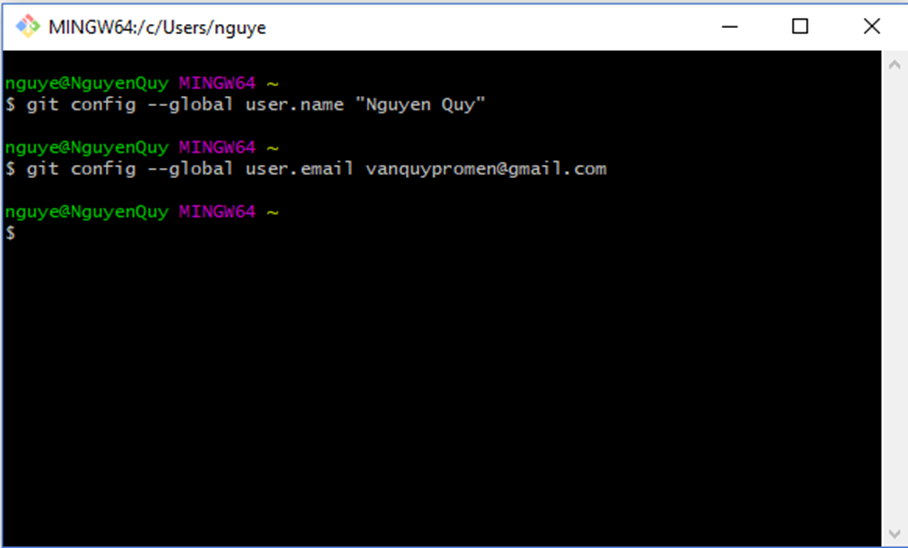
\includegraphics[width=0.8\linewidth]{screenshot001}
	\caption{Thiết lập username và useremail}
	\label{fig:screenshot001}
\end{figure}
	\end{itemize}
\end{itemize}

\subsection{Trình soạn thảo}
\begin{itemize}
\item Ở bước cài đặt Git, chúng ta đã chọn Visual Studio Code làm công cụ chỉnh sửa mặc định.
\item Nếu muốn thay đổi công cụ mặc định đã được cài đặt trước đó thì có thể sử dụng lệnh:
\textcolor{blue}{\bf git config \texttt{-{}-}global core.editor “ ’[đường dẫn đến công cụ trong máy bạn]’ -multilnst -nosession”}
\item Ví dụ: muốn cho Visual Studio Code làm công cụ soạn thảo mặc định cho Git
	\begin{figure}[!ht]
	\centering
	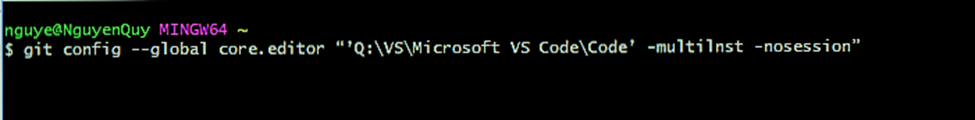
\includegraphics[width=0.8\linewidth]{screenshot002}
	\caption{Thay đổi công cụ}
	\label{fig:screenshot002}
\end{figure}
\end{itemize}


\subsection{Kiểm tra các cài đặt}
\begin{itemize}
\item Khi muốn kiểm tra các cài đặt, ta dùng lệnh \textcolor{blue}{\bf git config \texttt{-{}-}list}. Kết quả như hình bên dưới: 
\begin{figure}[!ht]
	\centering
	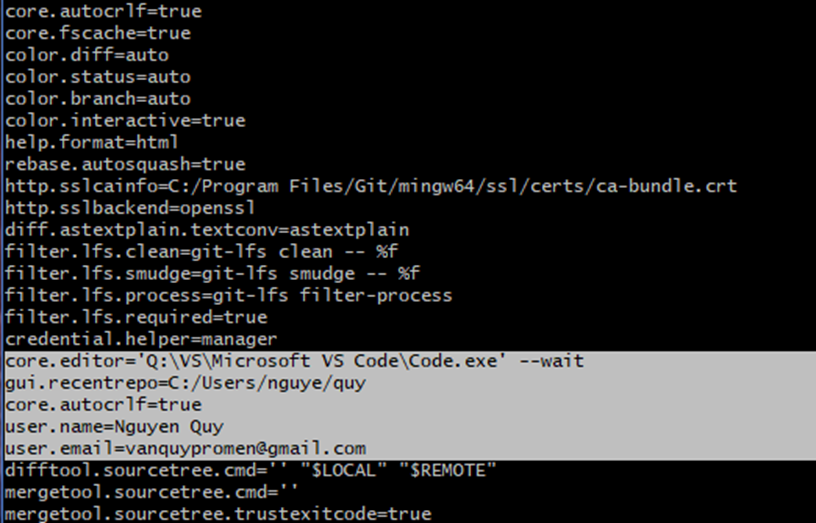
\includegraphics[width=0.8\linewidth]{screenshot003}
	\caption{Kiểm tra cài đặt}
	\label{fig:screenshot003}
	\end{figure}
\item Ta có thể kiểm tra giá trị của từng khoá riêng biệt bằng lệnh: \textcolor{blue}{\bf git config \{khoá\}}
\item Ví dụ như ta muốn xem tên người dùng và địa chỉ email, ta gõ lệnh như trong hình: 

\begin{figure}[!ht]
	\centering
	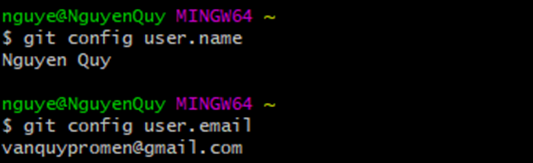
\includegraphics[width=0.8\linewidth]{screenshot004}
	\caption{Kiểm tra username và usermail}
	\label{fig:screenshot004}
\end{figure}

\item Git còn được trang bị các trang hướng dẫn cho các lệnh, hiển thị bằng cách
\begin{itemize}
\item \textcolor{blue}{\bf git help <lệnh>}
\item \textcolor{blue}{\bf git <lệnh> \texttt{-{}-}help}
\item \textcolor{blue}{\bf man git-<lệnh>}
\end{itemize}
 \end{itemize}
 
\section{Khởi tạo Repository}

\subsection{Khởi tạo một repository trong một thư mục có sẵn}
\begin{itemize}
\item Repository, hay còn gọi là Repo, trong tiếng Việt nghĩa là kho chứa. Repo là nơi chứa tất cả mã nguồn cho một dự án được quản lý bởi Git.
\item Nếu bạn muốn bắt đầu quản lý một dự án có sẵn bằng Git, bạn cần di chuyển đến thư mục đó sử dụng bash và gõ: \textcolor{blue}{\bf git init}
\item Để di chuyển đến thư mục, ta sử dụng lệnh: \textcolor{blue}{\bf cd <đường dẫn thư mục> }

\begin{figure}[!ht]
	\centering
	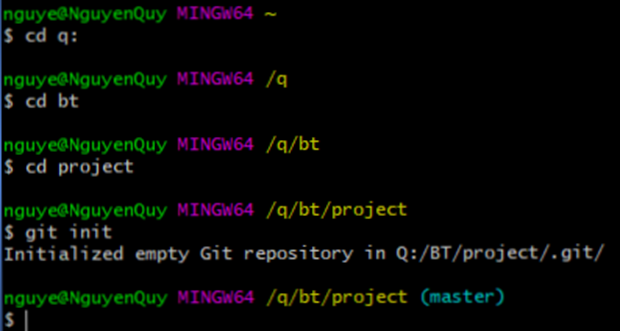
\includegraphics[width=0.8\linewidth]{screenshot005}
\caption{Tạo Repository}
	\label{fig:screenshot005}
\end{figure}

\item Ở hình trên, sử dụng lệnh cd để di chuyển đến thư mục project chứa bài tập lớn cần quản lý có đường dẫn là \textcolor{blue}{\bf Q:/BT/project} và sau đó sử lệnh \textcolor{blue}{\bf git init} để tạo ra một thư mục tên là .git, thư mục này chính bộ khung xương của Repo.
\end{itemize}
\subsection{Sao chép một Repo có sẵn}
\begin{itemize}
\item Nếu bạn muốn có một bản sao của một Git repo có sẵn, ví dụ như repo của một dự án mà bạn muốn tham gia, sử dụng lệnh \textcolor{blue}{\bf git clone <đường dẫn đến repo>}
\item Đường dẫn có thể là link dẫn đến kho lưu trữ mã nguồn của nhóm làm việc với bạn trên nền web như GitHub
\end{itemize}
\section{Quản lý Repository}

\subsection{Vòng tuần hoàn trạng thái của tệp}

\begin{figure}[!ht]
	\centering
	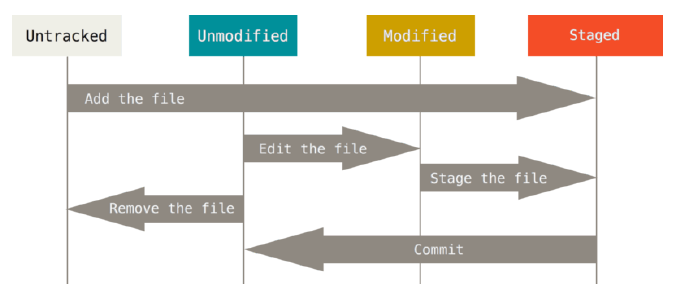
\includegraphics[width=0.8\linewidth]{screenshot006}
	\caption{Vòng tuần trạng thái}
	\label{fig:screenshot006}
	\end{figure}
\begin{itemize}
\item \textcolor{blue}{\bf Untracked}: tệp chưa được theo dõi (track)
\item \textcolor{blue}{\bf Unmodified}: tệp đã được commit
\item \textcolor{blue}{\bf Modified}: tệp đã được chỉnh sửa và chưa commit
\item \textcolor{blue}{\bf Staged}: các tệp đã được theo dõi hoặc các tệp đã chỉnh sửa đang chờ để commit
\end{itemize}
\subsection{Kiểm tra trạng thái của tệp}
\begin{itemize}
\item Lệnh \textcolor{blue}{\bf git status} dùng để kiểm tra trạng thái của thư mục đang làm việc hiện tại.
	\begin{itemize}
		\item Dưới đây, ta kiểm tra trạng thái của thư mục làm việc (working directory) hiện tại là project

\begin{figure}[!ht]
	\centering	
	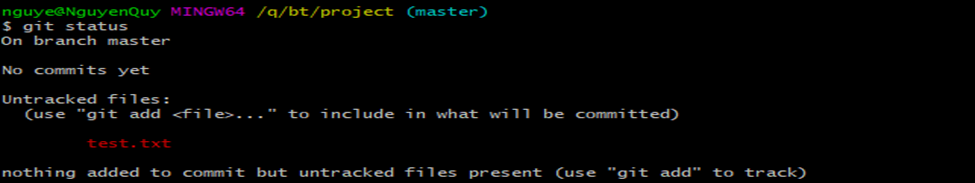
\includegraphics[width=0.8\linewidth]{screenshot007}
\caption{Kiểm tra trạng thái}
	\label{fig:screenshot007}
\end{figure}

		\item Ở hình trên, ta thấy tệp \textcolor{blue}{\bf test.txt} không được thêm vào Repo, đang ở trạng thái untracked (chưa được theo dõi)
	\end{itemize}
\item Để theo dõi một tập tin, ta dùng lệnh \textcolor{blue}{\bf git add <tên tệp>}, cụ thể ở đây ta theo dõi tệp \textcolor{blue}{\bf test.txt}

\begin{figure}[!ht]
	\centering
	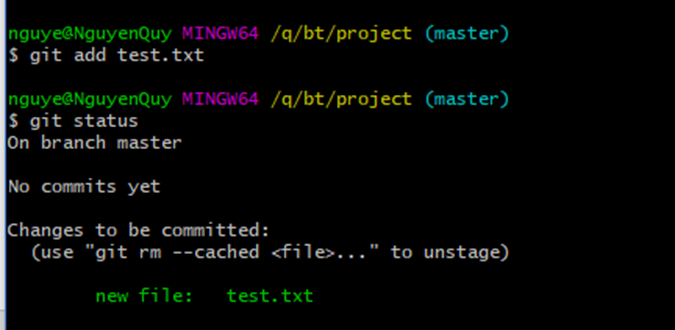
\includegraphics[width=0.8\linewidth]{screenshot008}
\caption{Thêm một tệp vào Staged}
	\label{fig:screenshot008}
	\end{figure}
\end{itemize}
\subsection{Bỏ qua các tập tin}
\begin{itemize}
\item Tệp \textcolor{blue}{\bf .gitignore} liệt kê những file mà mình không mong muốn cho vào Git (Git sẽ lờ những file đó đi)
\item Tạo file gitignore bằng lệnh \textcolor{blue}{\bf touch .gitignore}
\item Các pattern format hay dùng:
	\begin{itemize}
	\item Sử dụng \# để comment và có thể để cách dòng cho dễ đọc. 
	\item Đơn giản nhất là tên file cần ignore: example.exe, example.txt, …
	Hay cả thư mục: example\_folder/
	\item Sử dụng * để tìm các file có cùng định dạng. Ví dụ như bạn muốn Git bỏ qua tất cả các file .xml trong project: *.xml
	\end{itemize}
\item Ví dụ: 
\begin{itemize}
\item Trong Repo hiện tại có thư mục bin và ta muốn Git bỏ qua thư mục đó

\begin{figure}[!ht]
	\centering
	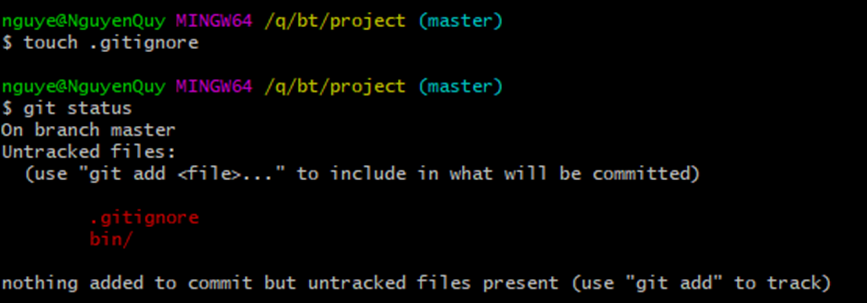
\includegraphics[width=0.8\linewidth]{screenshot009}
\caption{Thư mục /bin}
	\label{fig:screenshot009}
\end{figure}
\item Ta chỉnh sửa file \textcolor{blue}{\bf .gitignore }để thêm thư mục bin vào

\begin{figure}[!ht]
	\centering
	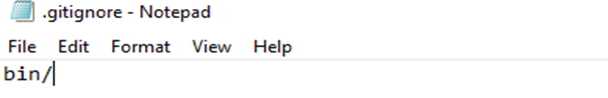
\includegraphics[width=0.8\linewidth]{screenshot010}
	\caption{Thêm vào \textcolor{blue}{\bf .gitignore }}
	\label{fig:screenshot010}
\end{figure}

\item Sau khi thêm bin vào \textcolor{blue}{\bf .gitignore}, ta kiếm tra lại trạng thái và thấy thư mục bin đã bị Git bỏ qua.

\begin{figure}[!ht]
	\centering
	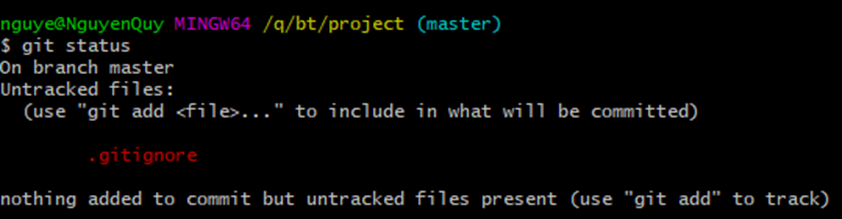
\includegraphics[width=0.8\linewidth]{screenshot011}
\caption{Kết quả}
	\label{fig:screenshot011}
	\end{figure}
	
\end{itemize}
\end{itemize}
\subsection{Xem các thay đổi} 
\begin{itemize}
\item Câu lệnh \textcolor{blue}{\bf git status} vẫn còn mơ hồ, ta không thể biết chính xác được cái gì đã được thay đổi
\item Lệnh \textcolor{blue}{\bf git diff} cho ta biết chính xác từng dòng được thêm vào hay xoá đi
\item Câu lệnh \textcolor{blue}{\bf git diff \texttt{-{}-}staged} đã được tổ chức (staged) và chuẩn bị được commit.
\end{itemize}
\subsection{Commit các thay đổi}
\begin{itemize}
\item Sau khi đã tổ chức các tập tin theo ý muốn, chúng ta có thể commit chúng
\item Lưu ý rằng những thứ chưa được tổ chức (unstaged) – những file được tạo ra hoặc chỉnh sửa sau khi bạn chạy lệnh \textcolor{blue}{\bf git add} sẽ không được commit, do những file vẫn đang ở trạng thái modified.
\item Cách đơn giản để commit đó là dùng lệnh: \textcolor{blue}{\bf git commit –m “message”}
	\begin{itemize}
	\item Sau khi đã đưa các tệp lên trạng thái staged ta phải sử dụng lệnh: \textcolor{blue}{\bf git commit -m “initial project version”} (initial project version chính là message, tóm tắt nội dung của lần commit này) để commit các tệp đang ở trạng thái staged

\begin{figure}[!ht]
	\centering
	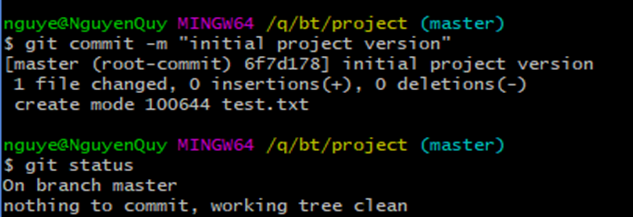
\includegraphics[width=0.8\linewidth]{screenshot012}
\caption{Thực hiện commit file}
	\label{fig:screenshot012}
\end{figure}
	\item Kết quả ta sẽ được như hình trên, tệp test.txt đã được commit.
\end{itemize}
\end{itemize}
\subsection{Bỏ qua khu vực tổ chức (staging area)}
\begin{itemize}
\item Thêm lựa chọn -a vào câu lệnh git commit sẽ làm Git tự động tổ chức (stage) tất cả những tệp đã được theo dõi trước khi thực hiện commit, cho phép ta bỏ qua bước \textcolor{blue}{\bf git add}
\item Có thế add hết tất cả các tệp untracked vào staged bằng lệnh: \textcolor{blue}{\bf git add \texttt{-{}-}all}

\begin{figure}[!ht]
	\centering
	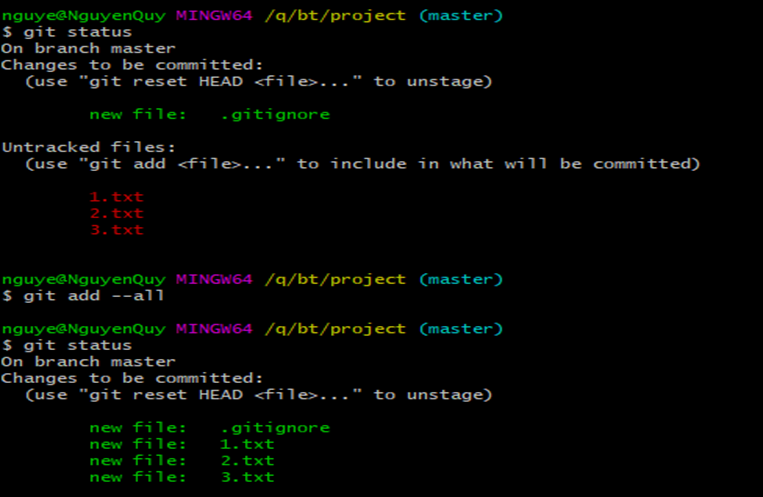
\includegraphics[width=0.8\linewidth]{screenshot013}
\caption{Thêm vào Staged}
	\label{fig:screenshot013}
\end{figure}

\item Ở hình trên, có 3 tệp tracked, sử dụng \textcolor{blue}{\bf git add \texttt{-{}-}all} để đưa cả 3 tệp vào stage area cùng lúc
\item Sau đó commit 1 lần 3 tệp trên bằng lệnh \textcolor{blue}{\bf git commit –a –m “commit flie”}, kết quả sẽ được như hình dưới

\begin{figure}[!ht]
	\centering
	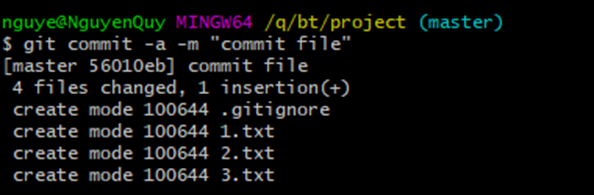
\includegraphics[width=0.8\linewidth]{screenshot014}
\caption{Kết quả sau commit}
	\label{fig:screenshot014}
	\end{figure}	
\end{itemize}

\subsection{Xoá tập tin} 
\begin{itemize}
\item \textcolor{blue}{\bf git rm}: Xoá một tập tin khỏi staging area, đồng thời cũng xoá tập tin đó trên ổ cứng.
\item \textcolor{blue}{\bf git rm \texttt{-{}-}cached} : tập tin không còn bị kiếm soát bởi Git nhưng mà vẫn còn trên ổ cứng

\begin{figure}[!ht]
	\centering
	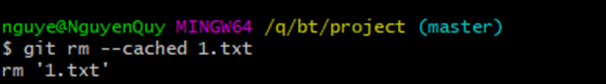
\includegraphics[width=0.8\linewidth]{screenshot015}
	\caption{Xóa tập tin}
	\label{fig:screenshot015}
	\end{figure}
	
\item Đổi tên tệp tin: Để đổi tên một tập tin trong Git, ta dùng lệnh sau: \textcolor{blue}{\bf git mv file\_from file\_to}

\begin{figure}[!ht]
	\centering
	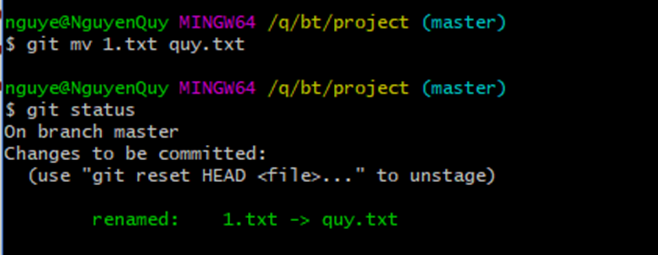
\includegraphics[width=0.8\linewidth]{screenshot016}
	\caption{Đổi tên}
	\label{fig:screenshot016}
	\end{figure}
\end{itemize}

\section{Xem lịch sử commit}
\begin{itemize}
\item Áp dụng khi xem lại các dòng code, các đoạn commit có sai sót gì, kiểm tra các đoạn chỉnh sửa những gì\vskip 0.4cm
\item Công cụ đơn giản và tốt nhất để thực hiện việc này là lệnh: \textcolor{blue}{\bf git log}

\begin{figure}[!ht]
	\centering
	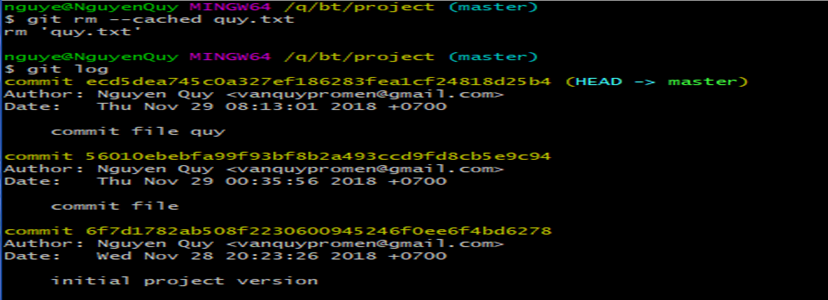
\includegraphics[width=0.8\linewidth]{screenshot017}
\caption{Xem lịch sử commit}
	\label{fig:screenshot017}
\end{figure}

\item Ở hình trên ta thấy Git đã hiển thị tất cả các lịch sử hoạt động của user. Ví dụ: Nguyen Quy đã commit file quy.txt vào 8:13 29/11/2018\vskip 0.4cm
\item Có rất nhiều tuỳ chọn khác nhau cho lệnh git log, giúp ta hiển thị thứ ta thực sự muốn
	\begin{itemize}
		\item Một trong những tuỳ chọn có ích nhất là -p : hiển thị sự khác nhau của từng commit. Có thể thêm -<x> để hiển thị x commit gần nhất. VD hiển thị sự khác nhau giữa 2 commit gần nhất: \textcolor{blue}{\bf git log –p -2}

\begin{figure}[!ht]
	\centering
	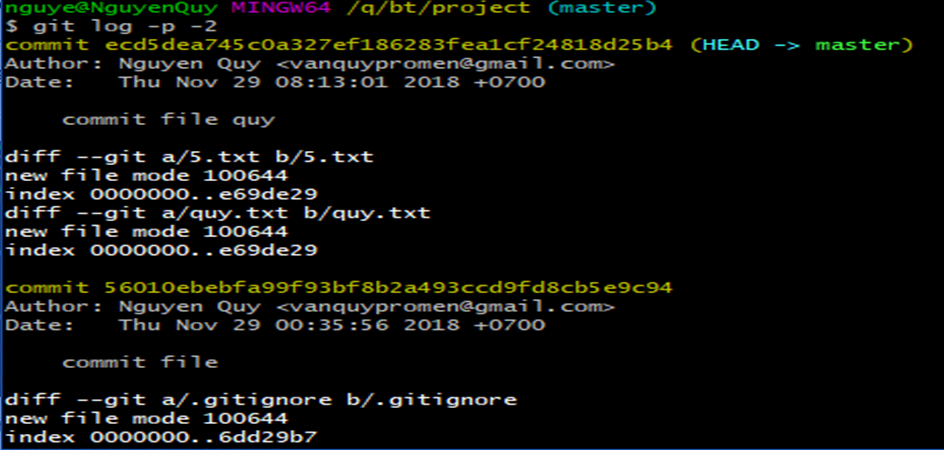
\includegraphics[width=0.8\linewidth]{screenshot018}
	\caption{Xem lịch sử có so sánh sự khác nhau}
	\label{fig:screenshot018}
\end{figure}

\item Ở hình trên chỉ hiển thị 2 hành động gần nhất nhưng có thêm một vài thông số. Ví dụ: bạn có thể sử dụng lệnh \textcolor{blue}{\bf diff \texttt{-{}-}git a/5.txt b/5.txt} để so sánh sự thay đổi của tệp 5.txt (a, b ở đây chỉ phiên bản của tệp)\vskip 0.4cm
\end{itemize}
\item Nếu ta muốn xem một bản thống kê tóm tắt cho mỗi commit, ta dùng lựa chọn \texttt{-{}-}stat. Lệnh \textcolor{blue}{\bf git log \texttt{-{}-}stat} sẽ in ra phía dưới mỗi commit danh sách các tập tin đã chỉnh sửa, bao nhiêu tập tin được sửa, và bao nhiêu dòng trong các tập tin đó được thêm vào hay xoá đi.

\begin{figure}[!ht]
	\centering
	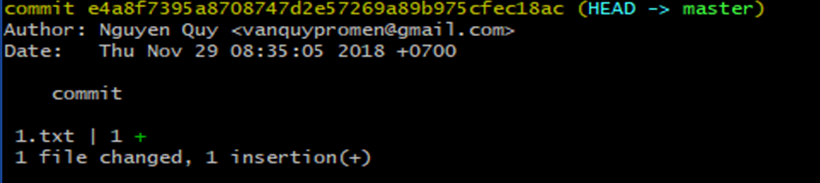
\includegraphics[width=0.8\linewidth]{screenshot019}
\caption{Hiển thị số tập tin, số dòng được chỉnh sửa}
	\label{fig:screenshot019}
	\end{figure}
	
\begin{itemize}
\item Như hình trên, Git đã hiện thị vào lần commit lúc 8:35 29/11, đã có 1 tệp thay đổi và tệp đó có thêm 1 dòng
\end{itemize}
\item Một lựa chọn hữu ích khác là \texttt{-{}-}pretty. Lựa chọn này thay đổi phần hiển thị theo các cách khác nhau.
\begin{itemize}
\item Lựa chọn oneline in ra mỗi commit trên một dòng, thuận tiện cho việc xem nhiều commit: \textcolor{blue}{\bf git log \texttt{-{}-}pretty=oneline}

\begin{figure}[!ht]
	\centering
	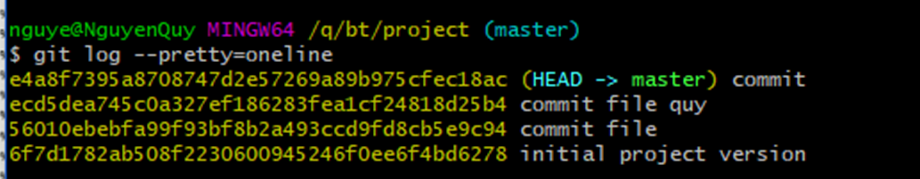
\includegraphics[width=0.8\linewidth]{screenshot020}
	\caption{Xem lịch sử một dòng}
	\label{fig:screenshot020}
	\end{figure}

\item Ta đã sử dụng \textcolor{blue}{\bf option \texttt{-{}-}pretty=oneline} để hiển thị mỗi commit chỉ là một dòng gồm commit ID và tin nhắn của mỗi lần commit
\end{itemize}
\item Lựa chọn thú vị nhất là \textcolor{blue}{\bf \texttt{-{}-}pretty=format}, cho phép ta chỉ định định dạng riêng của phần hiển thị.

\begin{figure}[!ht]
	\centering
	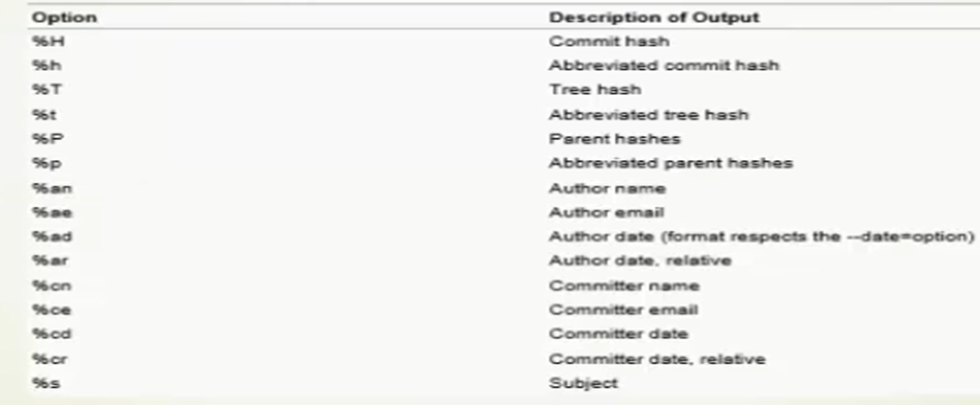
\includegraphics[width=0.8\linewidth]{screenshot021}
\caption{Bảng các thuộc tính cho \textcolor{blue}{\bf \texttt{-{}-}pretty=format}}
	\label{fig:screenshot021}
	\end{figure}

\begin{itemize}
\item Ví dụ: \textcolor{blue}{\bf git log \texttt{-{}-}pretty=format:”\%h - \%an, \%ar : \%s”}. Kết quả thu được

\begin{figure}[!ht]
	\centering
	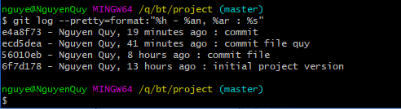
\includegraphics[width=0.8\linewidth]{screenshot022}
\caption{Hiển thị nâng cao}
	\label{fig:screenshot022}
	\end{figure}

\item Kết quả hiển thị commit ID thu gọn, tên tác giả, thời gian commit và tin nhắn cho mỗi lần commit. Với các option format này bạn có thể vận dụng cho việc báo cáo về tiến độ và kiểm soát làm việc cho từng thành viên
\end{itemize}
 \item Giới hạn thông tin đầu ra
\begin{itemize}
\item Các lựa chọn giới hạn thời gian thông tin đầu ra như \texttt{-{}-}since và \texttt{-{}-}until khá hữu ích

\begin{figure}[!ht]
	\centering
	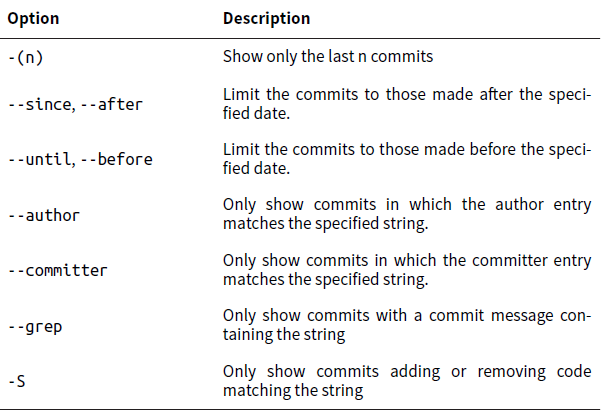
\includegraphics[width=0.8\linewidth]{screenshot023}
\caption{Bảng các thuộc tính giới hạng thông tin}
	\label{fig:screenshot023}
\end{figure}

\item Ví dụ: lệnh để hiển thị các commit từ 2 tuần trước trở lại do Nguyen Quy tạo ra:\textcolor{blue}{\bf git log \texttt{-{}-}pretty="\%h - \%s" \texttt{-{}-}author="Nguyen Quy" \texttt{-{}-}since=2.week }. Kết quả sẽ được:

\begin{figure}[!ht]
	\centering
	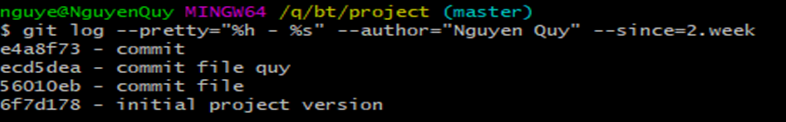
\includegraphics[width=0.8\linewidth]{screenshot024}
\caption{Kết quả thu được}
	\label{fig:screenshot024}
\end{figure}

\item Các option trên rất thích hợp cho bạn điều tra sai phạm trong dự án như là: tìm thấy người đã xóa tệp hay chỉnh sửa sai, thời gian xóa,…

\end{itemize}
\end{itemize}
	
\section{Hủy bỏ thay đổi}
\subsection{Undoing thing}
Khi bạn commit quá sớm và quên thêm các tệp khác hoặc bị lỗi phần message và muốn thử lại lần commit đó thì sử dụng: \textcolor{blue}{\bf git commit –amend}
\begin{itemize}
\item Ban đầu ta chỉ có một tệp 6.txt mới được tạo và ta muốn thêm vào commit với tin nhắn là “commit 1”

\begin{figure}[!ht]
	\centering
	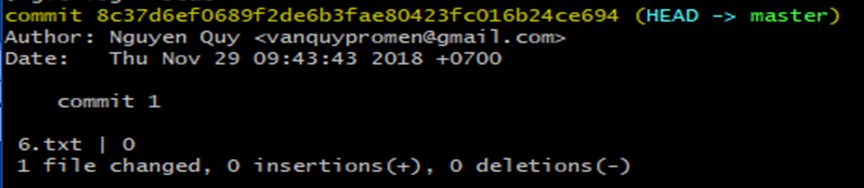
\includegraphics[width=0.8\linewidth]{screenshot026}
\caption{Tệp 6.txt được commit "commit 1"}
	\label{fig:screenshot026}
\end{figure}

\item Sau đó ta thêm 1 tệp 7.txt và không muốn tách ra làm 2 commit với tệp 6.txt mà muốn thêm vào “commit 1” trước đó với lệnh: \textcolor{blue}{\bf git commit \texttt{-{}-}amend}

\begin{figure}[!ht]
	\centering
	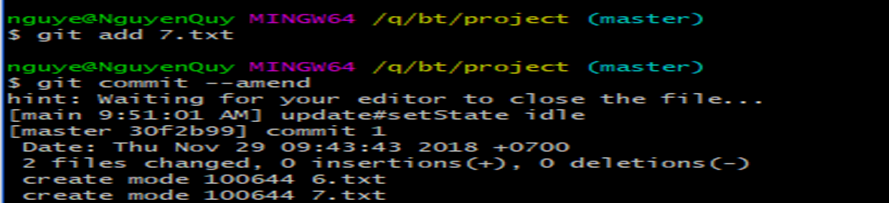
\includegraphics[width=0.8\linewidth]{screenshot027}
\caption{Commit tệp 7.txt vào "commit 1"}
	\label{fig:screenshot027}
	\end{figure}

\item Kết quả trong \textcolor{blue}{\bf git log} là:

\begin{figure}[!ht]
	\centering
	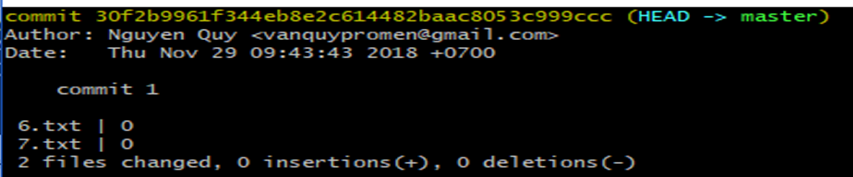
\includegraphics[width=0.8\linewidth]{screenshot028}
	\caption{Kết quả thu được}
	\label{fig:screenshot028}
	\end{figure}
\end{itemize}

\subsection{Unstaging a staged file}
\begin{itemize}
\item Giả sử bạn đã chỉnh sửa hai tệp và muốn commit từng chỉnh sửa riêng, nhưng bạn vô tình gõ \textcolor{blue}{\bf git add *} và tổ chức (staged) cả hai
\item Để unstage một tập tin: \textcolor{blue}{\bf git reset HEAD <name>}
	\begin{itemize}
\item Ví dụ: Hai tệp 1.txt và 2.txt đã được chỉnh sửa và đang ở trạng thái modified và thêm vào staged

\begin{figure}[!ht]
	\centering
	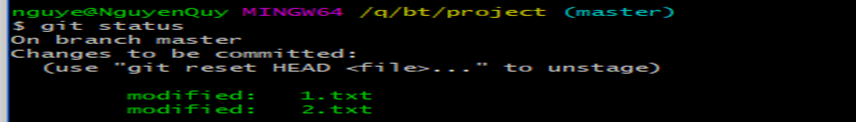
\includegraphics[width=0.8\linewidth]{screenshot029}
\caption{Tệp 1.txt và 2.txt}
	\label{fig:screenshot029}
	\end{figure}

\item Nhưng giờ bạn muốn chỉ commit tệp 1.txt ở đợt commit này thì bạn phải unstaging tệp 2.txt đã được staged bằng lệnh: \textcolor{blue}{\bf git reset HEAD 2.txt}. Kết quả sẽ là:

\begin{figure}[!ht]
	\centering
	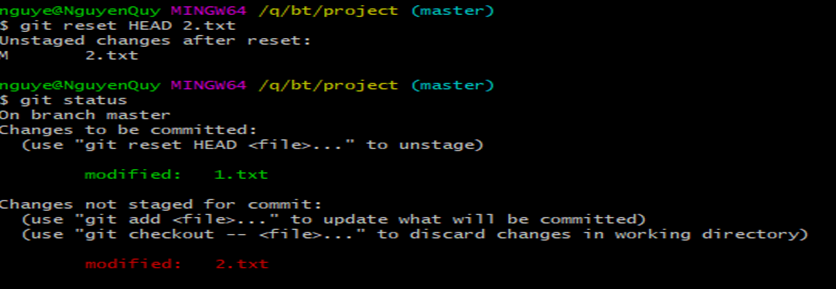
\includegraphics[width=0.8\linewidth]{screenshot030}
\caption{Unstaged tệp 2.txt}
	\label{fig:screenshot030}
	\end{figure}
	
\end{itemize}
\end{itemize}
\subsection{Unmodifying a modified file}
\begin{itemize}
\item Trong khi bạn làm việc, sẽ có những thay đổi trên tệp mà bạn không mong muốn, bạn muốn loại bỏ đi sự thay đổi đó để quay về với nội dung cũ thì sử dụng lệnh: \textcolor{blue}{\bf git checkout \texttt{-{}-}<tên tệp>}
\item Lưu ý rằng đây là một lệnh nguy hiểm – mọi thay đổi của bạn đối với tệp sẽ bị mất. Hãy chắc chắn là bạn thực sự muốn bỏ các thay đổi vừa thực hiện
	\begin{itemize}
\item Ví dụ: Tiếp nối ví dụ phía trên, ta đang có tệp 2.txt được chỉnh sửa, giờ bạn muốn loại bỏ đi sự thay đổi đó thì sử dụng lệnh: \textcolor{blue}{\bf git checkout \texttt{-{}-}2.txt}. Kết quả thu được

\begin{figure}[!ht]
	\centering
	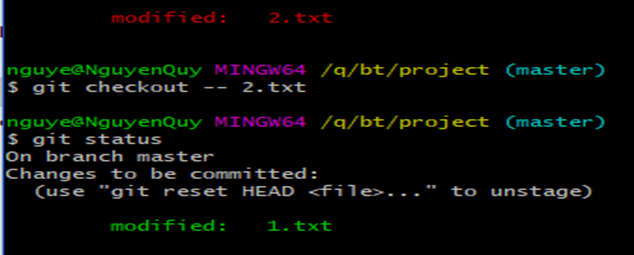
\includegraphics[width=0.8\linewidth]{screenshot031}
\caption{Bỏ đi các thay đổi trên 2.txt}
	\label{fig:screenshot031}
	\end{figure}

\item Tệp 2.txt đã quay trở lại trước khi thay đổi và Git thông báo không có sự thay đổi nào
\end{itemize}\end{itemize}

\section{Làm việc với remote repository}
\subsection{Tổng quan} 
\begin{itemize}
\item Để có thể cộng tác trên bất kỳ dự án nào với Git, bạn cần biết cách quản lý remote repo (kho lưu trữ từ xa) của mình
\item Remote repositories (Kho lưu trữ từ xa) là các phiên bản của dự án được lưu trữ trên Internet,  trên một máy chủ được được các tổ chức cung cấp
\item Cộng tác với những người khác liên quan đến việc quản lý remote repo này, đẩy dữ liệu lên và kéo dữ liệu  từ chúng khi bạn cần chia sẻ công việc
\item Quản lý remote repository bao gồm biết cách thêm, xóa các điều khiển từ xa không còn hợp lệ, quản lý các nhánh từ xa (remote branch) khác nhau và xác định chúng như đang được theo dõi hay không và hơn thế nữa
\end{itemize}
\subsection{Hiển thị remotes} 
\begin{itemize}
\item Để xem remote repo nào bạn đã cấu hình, bạn có thể chạy lệnh git remote
\item Nó liệt kê các tên ngắn của mỗi remote
\item Nếu bạn đã sao chép remote của mình, bạn nên xem nguồn gốc - đó là tên mặc định mà Git cung cấp cho máy chủ mà bạn đã sao chép. 
\item Ví dụ dưới đây ta clone một remote Repo trên github:
	\begin{itemize}
		\item \textcolor{blue}{\bf git clone https://github.com/nguyenquy43/first.git}
		\item \textcolor{blue}{\bf git remote} (xem thông tin remote repository bạn mới lưu về máy)

\begin{figure}[!ht]
	\centering
	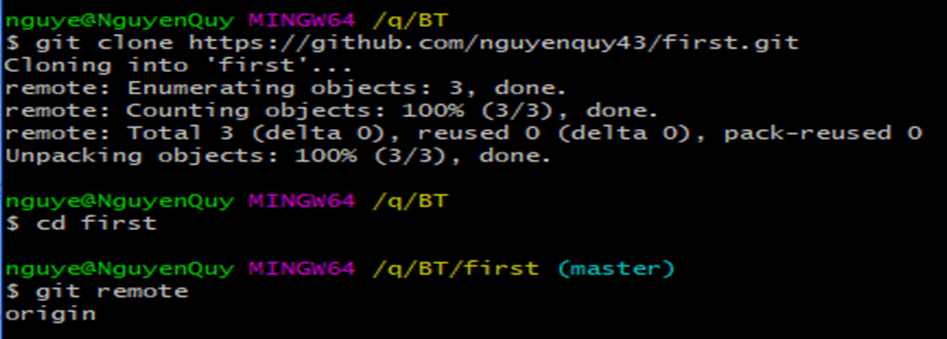
\includegraphics[width=0.8\linewidth]{screenshot032}
	\caption{Kết quả sau khi clone}
	\label{fig:screenshot032}
	\end{figure}
	\end{itemize}
\item Bạn có thể dùng –v để hiển thị URL mà Git đã lưu trữ cho tên ngắn được sử dụng khi đọc và ghi vào remote đó: \textcolor{blue}{\bf git remote -v}

\begin{figure}[!ht]
	\centering
	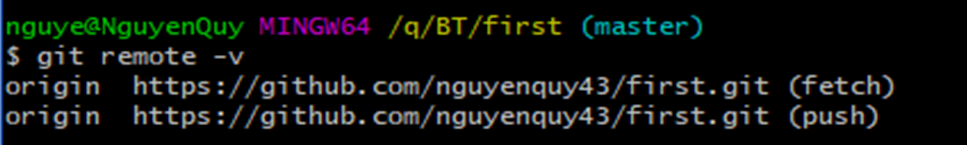
\includegraphics[width=0.8\linewidth]{screenshot033}
	\caption{Hiển thị URL}
	\label{fig:screenshot033}
\end{figure}
	\begin{itemize}
\item fetch là link để ta lấy dữ liệu từ remote, push là link để ghi dữ liệu lên remote
\end{itemize}\end{itemize}
\subsection{Thêm remote repository} 
\begin{itemize}
\item Khi bạn có sẵn một repository trong máy, và bạn muốn liên kết với một remote repository
\item Để thêm một remote repo mới dưới dạng một tên ngắn: \textcolor{blue}{\bf git remote add <shortname> <url>}
\item Ví dụ: 

\begin{figure}[!ht]
	\centering
	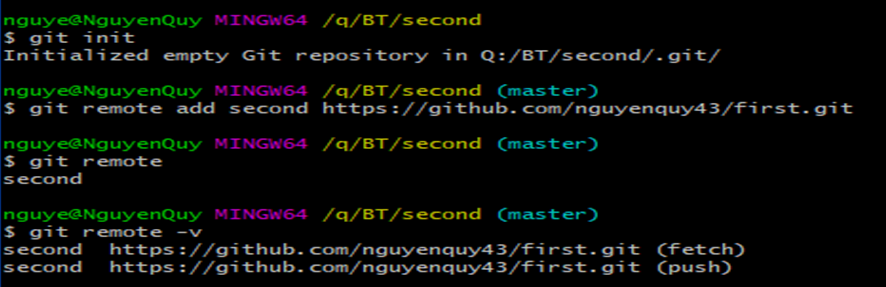
\includegraphics[width=0.8\linewidth]{screenshot034}
\caption{Thêm remote repo}	
	\label{fig:screenshot034}
	\end{figure}
\end{itemize}
\subsection{Nạp và kéo dữ liệu từ remote repository} 
\begin{itemize}
\item Lệnh đi đến remote repo và kéo tất cả dữ liệu từ remote repo mà bạn chưa có: \textcolor{blue}{\bf git fetch <remote name>}
\item Điều cần lưu ý là lệnh git fetch chỉ tải dữ liệu xuống  local repo của bạn - nó không tự động kết hợp (merge) dữ liệu đó với bất kỳ dữ liệu nào của bạn hoặc sửa đổi những gì bạn hiện đang làm việc
\item Bạn có thể sử dụng lệnh git pull để tự động tìm nạp và sau đó hợp nhất nhánh từ xa (remote branch) đó vào nhánh hiện tại của bạn: \textcolor{blue}{\bf git pull <remote name> <branch name>}
\item Ví dụ: 
	
	\begin{figure}[!ht]
	\centering
	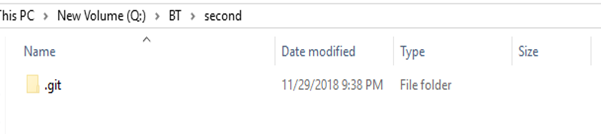
\includegraphics[width=0.8\linewidth]{screenshot035}
\caption{Local repo trước khi kéo (pull) dữ liệu}
	\label{fig:screenshot035}
	\end{figure}

\begin{figure}[!ht]
	\centering	
	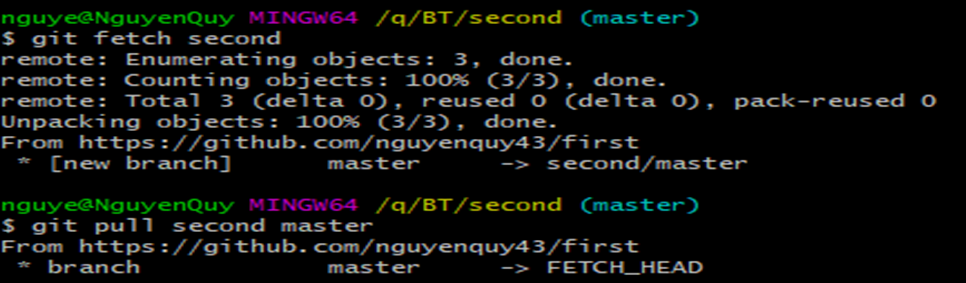
\includegraphics[width=0.8\linewidth]{screenshot036}
\caption{Thực hiện kéo dữ liệu}
	\label{fig:screenshot036}
\end{figure}

\begin{itemize}
\item Kết quả thu được là: 

\begin{figure}[!ht]
	\centering
	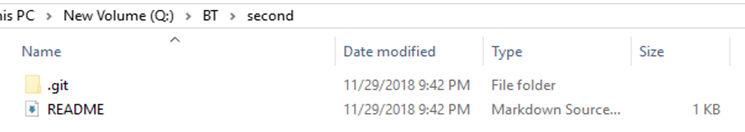
\includegraphics[width=0.8\linewidth]{screenshot037}
\caption{Kết quả}
	\label{fig:screenshot037}
\end{figure}

\item Tệp README đã được kéo về từ kho lữu trữ về second remote repository
\end{itemize}
\end{itemize}

\subsection{Đẩy lên remote repo}
\begin{itemize}
\item Khi bạn có một điểm trong dự án mà bạn muốn chia sẻ, bạn phải đẩy (pushing) bằng lệnh: \textcolor{blue}{\bf git push <remote name> <brach name> }
\item Lệnh này chỉ hoạt động nếu bạn nhân bản (clone) từ một máy chủ mà bạn có quyền truy cập ghi và không có ai đẩy trong thời gian đó
\item Ví dụ: Trong project second ta đã thêm một tệp text.txt và bây giờ ta cần thêm nó vào local repository và đưa nó lên kho dữ liệu

\begin{figure}[!ht]
	\centering
	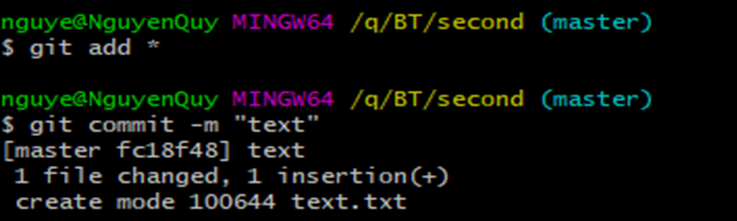
\includegraphics[width=0.8\linewidth]{screenshot038}
\caption{Commit text.txt}
	\label{fig:screenshot038}
\end{figure}

\item Sau khi đã commit, ta tiến hành đưa lên remote repository bằng lệnh: \textcolor{blue}{\bf git push second master}

\begin{figure}[!ht]
	\centering
	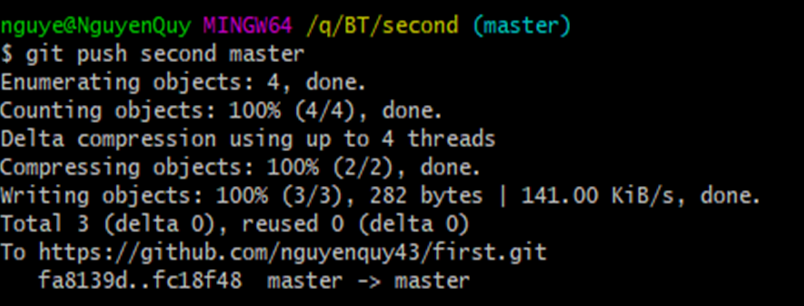
\includegraphics[width=0.8\linewidth]{screenshot039}
\caption{Đẩy (push) lên remote repo}
	\label{fig:screenshot039}
	\end{figure}
\end{itemize}	

\subsection{Kiểm tra ,xóa và đổi tên remotes} 
\begin{itemize}
\item Nếu bạn muốn xem thêm thông tin về một remote cụ thể: \textcolor{blue}{\bf git remote show <remote name>}

\begin{figure}[!ht]
	\centering	
	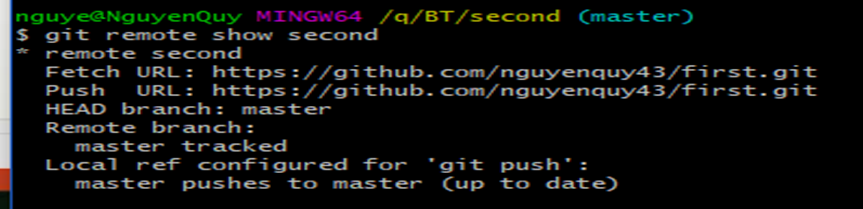
\includegraphics[width=0.8\linewidth]{screenshot040}
\caption{Xem thông tin remote cụ thể}
	\label{fig:screenshot040}
	\end{figure}

\item Bạn thay đổi shortname của remote: \textcolor{blue}{\bf git remote rename <old remote name> <new remote name>}
\item Nếu muốn loại bỏ remote repo  bạn có thể sử dụng: \textcolor{blue}{\bf git remote rm <remote name> }

\begin{figure}[!ht]
	\centering
	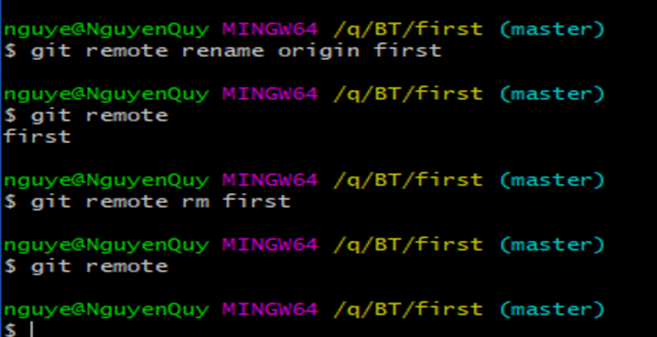
\includegraphics[width=0.8\linewidth]{screenshot041}
\caption{Loại bỏ remote repo}
	\label{fig:screenshot041}
	\end{figure}
\end{itemize}

			
\section{Làm việc với tag (thẻ) trong GIT}
\begin{itemize}
\item Như hầu hết các VCS, Git có khả năng gắn thẻ (tag) các điểm cụ thể quan trọng trong quá trình phát triển
\item Thông thường người sử dụng chức năng này dùng để các release point (đánh dấu những phiên bản và sau đó chỉ cần liệt kê theo tag đã đánh dấu để tìm những phiên bản đã được đánh dấu từ trước)
\end{itemize}
\subsection{Liệt kê, tạo thẻ}
\begin{itemize}
\item Liệt kê thẻ
	\begin{itemize}
		\item Liệt kê tất cả các thẻ của bạn: \textcolor{blue}{\bf git tag}
		\item Bạn có thể tìm kiếm các thẻ theo một yêu cầu nhất định. 
		\item Ví dụ, Git source repo chứa hơn 500 tags. Nếu bạn chỉ cần xem các thẻ có đầu là v.1.8.5git tag –l “v.1.8.5*”
	\end{itemize}
\item Tạo thẻ
	\begin{itemize}
		\item Git sử dụng hai loại thẻ chính: lightweight và annotated
		\item Một thẻ lightweight (thẻ nhẹ) nó chỉ trỏ đến một commit cụ thể: \textcolor{blue}{\bf git tag <tag name>-lw.}
		
		\begin{figure}[!ht]
	\centering
	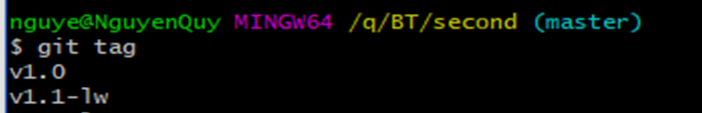
\includegraphics[width=0.8\linewidth]{screenshot042}
\caption{Tạo thẻ nhẹ}
	\label{fig:screenshot042}
\end{figure}

		\item Thẻ annotated (thẻ lưu trữ) được lưu trữ dưới dạng các đối tượng đầy đủ trong Git: \textcolor{blue}{\bf git tag –a <tag name> -m “message”}. Bạn có thể xem dữ liệu thẻ cùng với commit đã được gắn thẻ bằng cách sử dụng: \textcolor{blue}{\bf git show <tag name>}

\begin{figure}[!ht]
	\centering
	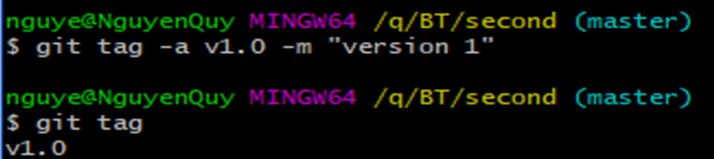
\includegraphics[width=0.8\linewidth]{screenshot043}
\caption{Tạo thẻ lưu trữ}
	\label{fig:screenshot043}
\end{figure}

		\item Bạn nên thường xuyên gắn thẻ có chú thích (annotted tag) để bạn có thể có tất cả thông tin này; nhưng nếu bạn muốn một thẻ tạm thời hoặc vì một lý do nào đó không muốn giữ thông tin khác hãy sử dụng thẻ lightweight
\end{itemize}
\end{itemize}
\subsection{Một số thao tác khác với thẻ}
\begin{itemize}
\item Bạn cũng có thẻ gắn thẻ các commit sau khi bạn đã di chuyển chúng. Để gắn thẻ commit đó:
\begin{itemize}
\item \textcolor{blue}{\bf git log \texttt{-{}-}pretty=oneline}: Lệnh này để xem lịch sử các commit ở dạng một dòng, dùng để lấy checksum ID của commit
\item Sau đó thì thì sử dụng lệnh: \textcolor{blue}{\bf git tag <tag name> <checksum ID>}
\item Ví dụ: 

\begin{figure}[!ht]
	\centering
	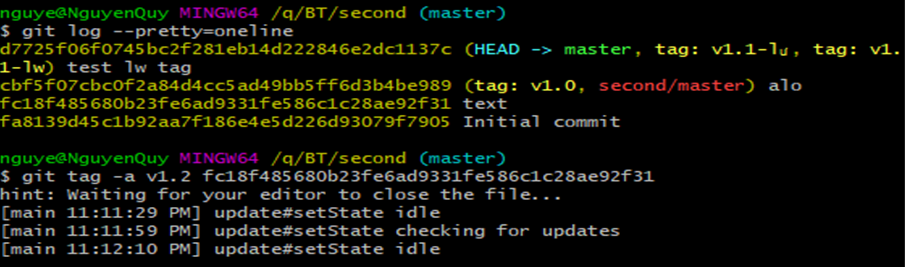
\includegraphics[width=0.8\linewidth]{screenshot044}
\caption{Xem thông tin thẻ}
	\label{fig:screenshot044}
	\end{figure}
	
\end{itemize}
\item Chia sẻ thẻ
\begin{itemize}
\item Lệnh \textcolor{blue}{\bf git push} không thể chuyển thẻ tới máy chủ
\item Bạn sẽ phải đẩy thẻ bằng một cách khác vào máy chủ với lệnh: \textcolor{blue}{\bf git push <remote name> <tag name>}
\item Nếu bạn có nhiều thẻ mà bạn muốn đẩy lên cùng một lúc: \textcolor{blue}{\bf git push <remote name> \texttt{-{}-}tags}
\item Ví dụ:

\begin{figure}[!ht]
	\centering
	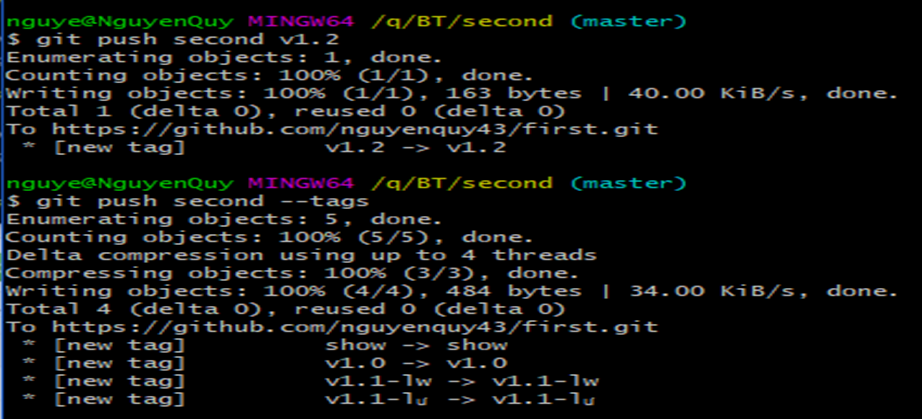
\includegraphics[width=0.8\linewidth]{screenshot045}
\caption{Chia sẻ thẻ lên remote repo}
	\label{fig:screenshot045}
	\end{figure}
	
\end{itemize}

\item Bạn không thể thực sự kiểm tra thẻ trong Git, vì chúng không thể di chuyển được. Nếu bạn muốn đặt một phiên bản của kho lưu trữ trong thư mục làm việc của bạn trông giống như một thẻ cụ thể, bạn có thể tạo một chi nhánh mới tại một thẻ cụ thể với : \textcolor{blue}{\bf git checkout –b <branchname> <tagname>}
\begin{itemize}
 \item Ví dụ: Ta có thể tạo mới một nhánh riêng có tag v1.2

\begin{figure}[!ht]
	\centering
	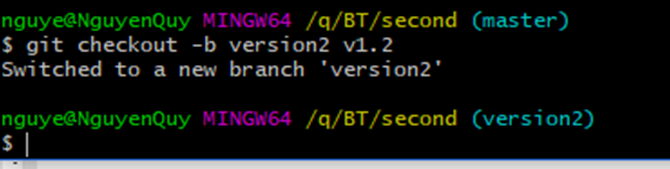
\includegraphics[width=0.8\linewidth]{screenshot046}
\caption{Tạo nhánh với một tag}
	\label{fig:screenshot046}
\end{figure}

\end{itemize}
\item Xóa thẻ
\begin{itemize}
\item Xóa thẻ ở kho dữ liệu trên máy bạn (local repo): \textcolor{blue}{\bf  git tag –d <tag name>}
\item Xóa thẻ trên máy chủ lưu trữ: \textcolor{blue}{\bf git push <remote name> \texttt{-{}-}delete <tag name>}

\begin{figure}[!ht]
	\centering
	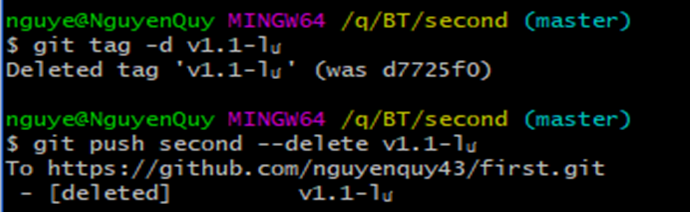
\includegraphics[width=0.8\linewidth]{screenshot047}
	\caption{Xóa thẻ}
	\label{fig:screenshot047}
	\end{figure}
	
\end{itemize}\end{itemize}
			
\section{Phân nhánh (branching)}
\begin{itemize}
\item Phân nhánh nghĩa là bạn tách khỏi dòng phát triển chính của dự án và tiếp tục làm việc mà không gây rối tới dòng chính đó (dùng để phát triển tính năng cho các phần mềm không gây ảnh hưởng)\vskip 0.4cm
\item Hiểu và nắm vững tính năng này cung cấp cho bạn một công cụ mạnh mẽ và độc đáo, hoàn toàn có thể thay đổi cách bạn phát triển các dự án
\end{itemize}
\subsection{Tạo một nhánh mới}
\begin{itemize}
\item Tạo một nhánh mới bằng lệnh: \textcolor{blue}{\bf git branch <branch name>}
\item Ví dụ: tạo một branch có tên là testing: \textcolor{blue}{\bf git branch testing}. Điều này tạo ra một con trỏ mới cho cùng một commit mà bạn đang thực hiện

\begin{figure}[!ht]
	\centering
	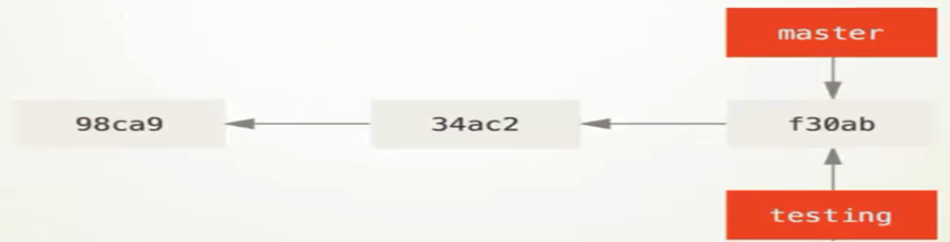
\includegraphics[width=0.8\linewidth]{screenshot051}
\caption{Sơ đồ các nhánh}
	\label{fig:screenshot051}
\end{figure}

\end{itemize}
\subsection{Con trỏ HEAD đến nhánh}
\begin{itemize}
\item Làm thế nào để Git biết bạn hiện đang thao tác ở nhánh nào? Nó được biểu diễn bằng một con trỏ đặc biệt: HEAD
\item Bạn có thể thấy được HEAD đang trỏ tới nhánh nào bằng lệnh: \textcolor{blue}{\bf git log \texttt{-{}-}oneline \texttt{-{}-}decorate}

\begin{figure}[!ht]
	\centering
	\includegraphics[width=0.8\linewidth]{screenshot052}
	\caption{Sơ đồ hiển thị vị trí HEAD}
	\label{fig:screenshot052}
	\end{figure}

\item Ví dụ

\begin{figure}[!ht]
	\centering
	\includegraphics[width=0.8\linewidth]{screenshot053}
	\caption{Xem vị trí HEAD}
	\label{fig:screenshot053}
	\end{figure}

\item Chuyển nhánh để di chuyển HEAD trỏ vào nhánh được chỉ định: \textcolor{blue}{\bf git checkout <branch name>} 
\item Ví dụ: \textcolor{blue}{\bf git checkout testing} -> chuyển HEAD trỏ sang nhánh testing

\begin{figure}[!ht]
	\centering
	\includegraphics[width=0.8\linewidth]{screenshot054}
\caption{Chuyển con trỏ HEAD}
	\label{fig:screenshot054}
\end{figure}

\end{itemize}
\subsection{Quản lý nhánh}
\begin{itemize}
\item Bạn có thể nhận được một danh sách nhánh hiện tại bằng lệnh: \textcolor{blue}{\bf git branch}

\begin{figure}[!ht]
	\centering
	\includegraphics[width=0.8\linewidth]{screenshot055}
	\caption{Xem danh sách nhánh}
	\label{fig:screenshot055}
\end{figure}

\item Lưu ý ký tự * đứng trước nhánh master: nó chỉ ra nhánh mà bạn hiện đã thao tác (nhánh mà HEAD trỏ tới)
\item Để xem lần commit cuối cùng trên mỗi nhánh: \textcolor{blue}{\bf git branch –v}
\item Các tùy chọn \texttt{-{}-}merged và \texttt{-{}-}no-merged có thể lọc danh sách gồm các nhánh đã hoặc chưa được kết hợp (merge) vào nhánh hiện đang truy cập: \textcolor{blue}{\bf git branch \texttt{-{}-}merged} và\textcolor{blue}{\bf git branch \texttt{-{}-}no-merged}

\begin{figure}[!ht]
	\centering
	\includegraphics[width=0.8\linewidth]{screenshot056}
\caption{Xem các nhánh đã và chưa kết hợp (merge)}
	\label{fig:screenshot056}
\end{figure}

\item Nếu bạn thật sự muốn xóa một nhánh và công việc đang thực hiện trên nhánh đó thì có thể sử dụng lệnh: \textcolor{blue}{\bf git branch –D <branch name>}

\begin{figure}[!ht]
	\centering
	\includegraphics[width=0.8\linewidth]{screenshot057}
\caption{Xóa một nhánh}
	\label{fig:screenshot057}
\end{figure}

\end{itemize}
\subsection{Phân nhánh luồng công việc} 
\begin{itemize}
\item Long-running branches (nhánh dài hạn): là các nhánh chính, đi xuyên suốt trong quá trình phát triển dự án
\begin{itemize}
\item Vì Git sử dụng một three-way merge đơn giản (là kết hợp 3 lần commit), việc hợp nhất từ nhánh này sang nhánh khác trong thời gian khác rất dễ thực hiện
\item Điều này có nghĩa là bạn có thể có nhiều nhánh luôn mở và bạn sử dụng cho các giai đoạn khác nhau trong chu kỳ phát triển dự án; bạn có thể thường xuyên merge (kêt hợp) từ một số nhánh trong số đó thành nhánh khác

\begin{figure}[!ht]
	\centering
	\includegraphics[width=0.8\linewidth]{screenshot058}
\caption{Sơ đồ phát triển các nhánh}
	\label{fig:screenshot058}
	\end{figure}
\end{itemize}
\item Topic branches (nhánh ngắn hạn): các nhánh thường được tạo ra với mục đích sửa lỗi, sau khi sửa lỗi không mà được merge với nhánh chính thì sẽ bị xóa

\begin{figure}[!ht]
	\centering
	\includegraphics[width=0.8\linewidth]{screenshot059}
				\caption{Nhánh ngắn hạn}	
						\label{fig:screenshot059}
\end{figure}

\item[$\nabla$]Quan trọng: Khi bạn đang branching (phân nhánh) và kết hợp (merging), mọi thứ chỉ được thực hiện trong kho lưu trữ Git của bạn (local repo) - không có giao tiếp với máy chủ nào đang diễn ra
\end{itemize}				
					
\section{Hợp (merge) nhánh và xử lý xung đột (conflicts)}

Merge branch tức là bạn gộp hai branch lại với nhau, thao tác này thường dùng để merge branch khác vào branch master trước khi push lên remote repository, hoặc merge hai branch thành một để giải quyết chung một task.	
\subsection{Basic merging}
\begin{itemize}
 \item Hãy tích hợp thay đổi đã thực hiện trên branch issue1 vào branch master

\begin{figure}[!ht]
	\centering
	\includegraphics[width=0.4\linewidth]{screenshot060}
\caption{Sơ đồ hai nhánh master và issue1}
	\label{fig:screenshot060}	
\end{figure}

\item Merge 2 nhánh sẽ được thực hiện bằng lệnh merge: \textcolor{blue}{\bf git merge <branch name>.}
\item Đầu tiên, sử dụng lệnh git checkout master để chuyển con trỏ HEAD đến nhánh master	
\item Tệp được chỉnh sửa là tệp issue.txt có nội dung: \textcolor{blue}{\bf "Đây là nội dung gốc"}	
\item Chỉnh sửa tệp issue.txt trong branch issue1: \textcolor{blue}{\bf "Đây là nội dung chỉnh sửa"}
\item Ta thực hiện tích hợp sự thay đổi trong tệp issue.txt giữa 2 nhánh

\begin{figure}[!ht]
	\centering	
	\includegraphics[width=0.8\linewidth]{screenshot01}
\caption{Tích hợp thay đổi}
	\label{fig:screenshot01}
\end{figure}

\begin{figure}[!ht]
	\centering
	\includegraphics[width=0.4\linewidth]{screenshot062}
\caption{Sơ đồ sau tích hợp}
	\label{fig:screenshot062}
	\end{figure}

\item Nội dung của tệp issue.txt sau merge:	

\begin{figure}[!ht]
	\centering
\includegraphics[width=0.8\linewidth]{screenshot02}
\caption{Nội dung issue.txt sau tích hợp}
	\label{fig:screenshot02}
	\end{figure}

\end{itemize}

\subsection{Basic merge conflicts}
\begin{itemize}
\item Giả sử, có 2 người đang cùng sửa 1 lỗi trên tệp issue.txt tại 2 branch khác nhau là issue2 và issue3	
\item Bây giờ, hãy tích hợp thay đổi tại branch issue2 và thay đổi tại branch issue3 vào master.
\item Trước tiên, sau khi đã checkout trên branch master, thực hiện merge branch issue2.	

\begin{figure}[!ht]
	\centering
	\includegraphics[width=0.8\linewidth]{screenshot03}
\caption{Merge branch issue2 và master}
	\label{fig:screenshot03}
	\end{figure}
\newpage
\item Như vậy merge fast-forward (chuyển tiếp nhanh) sẽ được thực hiện.	

\begin{figure}[!ht]
	\centering
	\includegraphics[width=0.8\linewidth]{screenshot063}
\caption{Sơ đồ sau merge}
	\label{fig:screenshot063}
	\end{figure}
	
\item Tiếp theo, thực hiện merge branch issue3	

\begin{figure}[!ht]
	\centering
	\includegraphics[width=0.8\linewidth]{screenshot04}
\caption{Merge branch issue3 và master}
	\label{fig:screenshot04}
	\end{figure}

\item Tự động merge đã thất bại. Có vẻ như đã phát sinh xung đột do đã thay đổi cùng một dòng với nội dung khác. Nội dung của issue.txt lúc này thì sẽ giống như bên dưới.

\begin{figure}[!ht]
	\centering
	\includegraphics[width=0.8\linewidth]{screenshot05}
\caption{Nội dung issue.txt sau khi merge thất bại}
	\label{fig:screenshot05}	
\end{figure}

\item Ở những chổ có xung đột thì Git đang chèn vào phần khác biệt. Hãy sửa như bên dưới.	

\begin{figure}[!ht]
	\centering
	\includegraphics[width=0.8\linewidth]{screenshot06}
\caption{Chỉnh sửa}
	\label{fig:screenshot06}	
\end{figure}

\item Vì đã chỉnh sửa nơi xung đột nên hãy commit lại.
\item Lịch sử sẽ giống thế này. Vì đã chỉnh sửa nơi xung đột trong merge lần này, nên merge commit sẽ ghi lại thay đổi đó sẽ được tạo mới. Và, đầu của master sẽ di chuyển đến đó. Loại merge thế này là không phải fast-forward mà được gọi là non fast-forward merge.

\begin{figure}[!ht]
	\centering
	\includegraphics[width=0.8\linewidth]{screenshot064}
\caption{Commit lại thay đổi trên issue.txt}
	\label{fig:screenshot064}
	\end{figure}
\end{itemize}

\section{Remote branches}
\subsection{Thiết lập ví dụ}
\begin{itemize}
\item Tại đường dẫn \textcolor{blue}{\bf /q/BT/example/remote} tạo một remote repo trên máy local bằng lệnh \textcolor{blue}{\bf git init \texttt{-{}-}bare}
\item Ta có một local repo tên local với snapshot như hình

\begin{figure}[!ht]
	\centering	
	\includegraphics[width=0.8\linewidth]{screenshot065}
	\caption{Sơ đồ snapshot}
	\label{fig:screenshot065}
\end{figure}

\item Tiến hành thiết lập remote cho nó bằng lệnh: \textcolor{blue}{\bf git remote add <remote  name> <address>} đặt tên remote là origin với địa chỉ là \textcolor{blue}{\bf /q/BT/example/remote}

\begin{figure}[!ht]
	\centering
	\includegraphics[width=0.8\linewidth]{screenshot066}
\caption{Thiết lập remote}
	\label{fig:screenshot066}
	\end{figure}
	
\item Tiến hành push tất cả dữ liệu từ repo local lên remote repo: \textcolor{blue}{\bf git push \texttt{-{}-}all origin}

\begin{figure}[!ht]
	\centering
	\includegraphics[width=0.8\linewidth]{screenshot07}
\caption{Push dữ liệu từ local lên remote}
	\label{fig:screenshot07}
	\end{figure}

\item Clone (nhân bản) từ remote repo: \textcolor{blue}{\bf git clone <address remote repo> <address clone>}
\item Các ví dụ sẽ được lấy từ repo clone
\item Trong một Local Repo, nếu Remote đặt tên là remotename, và một nhánh tên là branchname thì để biểu thị nhánh này trên Remote sẽ ký hiệu là remotename/branchename. Trạng thái sau khi nhân bản (clone)
\end{itemize}
\subsection{Trạng thái của của remote và clone}
\begin{itemize}
\item Kiểm tra trạng thái của repo clone

\begin{figure}[!ht]
	\centering
 	\includegraphics[width=0.8\linewidth]{screenshot067}
 \caption{Kiểm tra trạng thái repo}
 	\label{fig:screenshot067}
\end{figure}

\item Trạng thái của remote:

\begin{figure}[!ht]
	\centering
 	\includegraphics[width=0.8\linewidth]{screenshot068}
\caption{Trạng thái của remote}
 	\label{fig:screenshot068}
\end{figure}

\item Nhánh master của cả 2 đều đang ở snapshot C2
\end{itemize}
\subsection{Sự phân nhánh tại Local khi Remote cập nhật} 
\begin{itemize}
\item Giả sử ở repo local, có thêm 2 commit mới là snapshot C3, C4, sau đó cập nhật nhánh master lên remote: \textcolor{blue}{\bf git push origin master}

\begin{figure}[!ht]
	\centering
 	\includegraphics[width=0.8\linewidth]{screenshot069}
\caption{Sơ đồ sau khi push}
 	\label{fig:screenshot069}
\end{figure}

\begin{figure}[!ht]
	\centering
 	\includegraphics[width=0.8\linewidth]{screenshot070}
 \caption{Trạng thái sau khi push}
 	\label{fig:screenshot070}
 	\end{figure}
 	
\item Quay lại với repo clone, ta cũng tạo 2 commit C5, C6 nhưng không đẩy lên remote: ta thấy nhánh master 
 
\begin{figure}[!ht]
	\centering
 	\includegraphics[width=0.8\linewidth]{screenshot071}
 \caption{Sơ đồ snapshot tại master}
 	\label{fig:screenshot071}
 	\end{figure}
 
\begin{figure}[!ht]
	\centering 
 	\includegraphics[width=0.8\linewidth]{screenshot072}
 \caption{Trạng thái ở nhánh master}
 	\label{fig:screenshot072}
 	\end{figure}

\item Tiếp theo, sử dụng lệnh \textcolor{blue}{\bf git fetch \texttt{-{}-}all} để  tìm trong origin những dữ liệu mới sau đó cập nhật dữ liệu vào repo clone và kiểm tra trạng thái

\begin{figure}[!ht]
	\centering
 	\includegraphics[width=0.8\linewidth]{screenshot073}
 \caption{Cập nhật dữ liệu cho clone từ origin}
 	\label{fig:screenshot073}
 	\end{figure}

\item Nó cho biết nhánh master và origin/master tại repo colne bị phân nhánh. Có thể chuyển xem log của origin/master

\begin{figure}[!ht]
	\centering
 	\includegraphics[width=0.8\linewidth]{screenshot074}
 \caption{Log của nhánh origin/master}
 	\label{fig:screenshot074}
\end{figure}

\item Qua đó dựng được tình trạng master và origin/master bị phân ly ở repo clone như sau:

\begin{figure}[!ht]
	\centering
 	\includegraphics[width=0.8\linewidth]{screenshot075}
 \caption{Phân ly giữa master và origin/master}
 	\label{fig:screenshot075}
 	\end{figure}
\end{itemize}
\subsection{Pull – Hợp nhánh bị phân ly}
\begin{itemize}
\item Để hợp nhánh phân ly trên dùng lệnh merge để hợp nhánh origin/master vào master sau khi fetch dữ liệu về
\item Quá trình trên có thể tự động luôn cả 2 (tức là fetch xong, merge luôn) bằng lệnh git pull origin master
\item  Sau khi pull kiểm tra log:
 
\begin{figure}[!ht]
	\centering
 \includegraphics[width=0.8\linewidth]{screenshot076}
 	\label{fig:screenshot076}
\caption{Trạng thái sau khi pull}
\end{figure}

\begin{figure}[!ht]
	\centering
 	\includegraphics[width=0.8\linewidth]{screenshot077}
\caption{Sơ đồ snapshot sau khi pull}
 	\label{fig:screenshot077}
 	\end{figure}

\item Xóa nhánh tại remote: \textcolor{blue}{\bf git push remotename \texttt{-{}-}delete branchname}
 
\item Đổi tên nhánh local và remote
\begin{itemize}
	\item Đổi tên ở Local: \textcolor{blue}{\bf git branch -m old\_branch new\_branch}
  	\item Xóa nhánh ở Remote: \textcolor{blue}{\bf git push origin :old\_branch}
  	\item Cập nhật nhánh có tên mới lên  Remote: \textcolor{blue}{\bf git push \texttt{-{}-}set-upstream origin new\_branch}
\end{itemize}
\item Cập nhật nhánh mới từ remote vào local
 	\begin{itemize}
 	\item Cập nhật thông tin từ Remote: \textcolor{blue}{\bf git pull origin}
	\item Liệt kê các nhánh ở Remote: \textcolor{blue}{\bf git branch -r}
  	\item Tạo nhánh mới ở Local theo Remote: \textcolor{blue}{\bf git checkout -b branchname  origin/branchname}
 \end{itemize}\end{itemize}

\newpage

\chapter{Tổng kết} % Chương 3

Trên đây  là toàn bộ kiến thức mà nhóm đã học được trong thời gian tìm hiểu về GIT, qua đó nhóm đã thấy được nhưng lợi ích của GIT trong quá trình học tập và làm việc, đặc biệt là trong quá trình làm việc nhóm hay giải quyết những dự án lớn:
\begin{itemize}
\item Sắp xếp công việc tốt hơn
\item Linh hoạt hơn khi cùng phải làm cùng lúc nhiều task
\item Tự tin hơn khi thử nghiệm những ý tưởng mới
\item GitHub Community Forum là nơi để lập trình viên trao đổi, hỗ trợ và học hỏi với hơn 439000 developers và 1 triệu 350 ngàn repositories, đây chính là nơi hỗ trợ cho những bạn mới bắt đầu với git.
\end{itemize}

\begin{thebibliography}{99} % Tài liệu tham khảo

%\addcontentsline{toc}{chapter}{{\bf Tài liệu tham khảo}\rm}

\bibitem{Eva} Sách {\it Pro Git 2nd Edition} của tác giả Scott Chacon và Ben Straub

\bibitem{BaI} Các nguồn tài liệu trên mạng và youtube.

% Chú thích: mỗi tài liệu là một bibitem.

\end{thebibliography}

\end{document}